\chapter{First iteration prototypes}
\section{First group of sketches}
%First block of pictures
\begin{figure}[H]
		\centering
		\begin{subfigure}[b]{0.48\textwidth}
			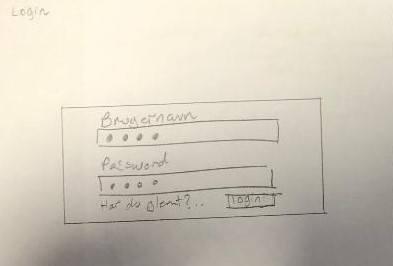
\includegraphics[width=\textwidth]{billeder/login-view.jpg}
			\caption{Login interface}
			\label{fig:1-Login}
		\end{subfigure}
		\quad
		\begin{subfigure}[b]{0.48\textwidth}
			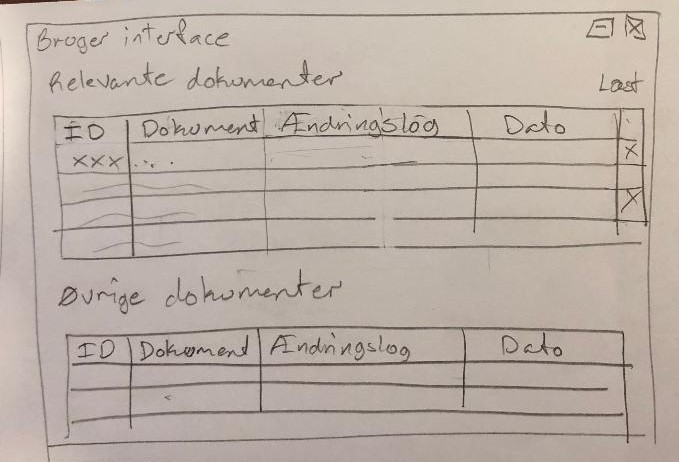
\includegraphics[width=\textwidth]{billeder/Main-view.jpg}
			\caption{Main page interface}
			\label{fig:1-Main}
		\end{subfigure}
\end{figure}
\begin{figure}[H]\ContinuedFloat
		\centering
		\begin{subfigure}[b]{0.48\textwidth}
			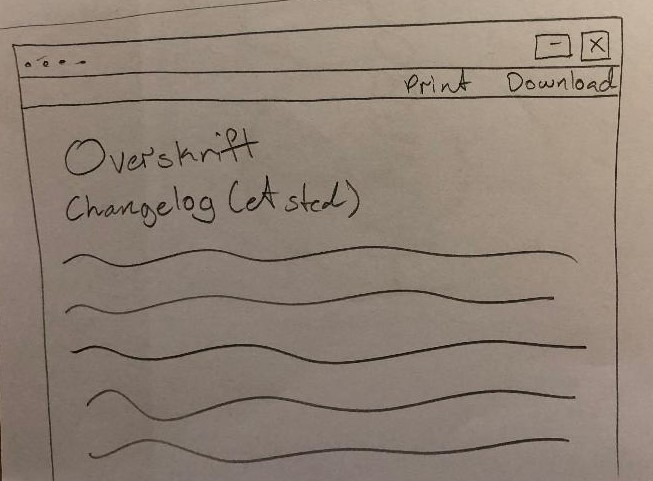
\includegraphics[width=\textwidth]{billeder/pdf-view.jpg}
			\caption{Pdf interface}
			\label{fig:1-pdf}
		\end{subfigure}
		\quad
		\begin{subfigure}[b]{0.48\textwidth}
			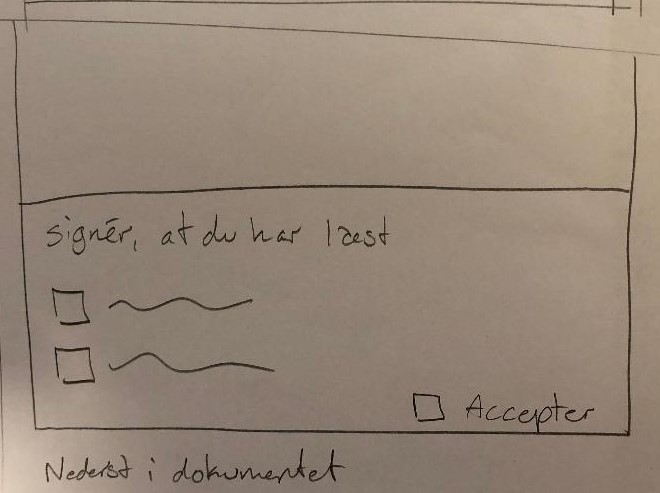
\includegraphics[width=\textwidth]{billeder/bottom-pdf-view.jpg}
			\caption{bottom of pdf view}
			\label{fig:1-bottom-pdf}
		\end{subfigure}
		\caption{Main interfaces and its connections}\label{fig:animals}
\end{figure}

%Second block of pictures
\begin{figure}[H]
	\centering
		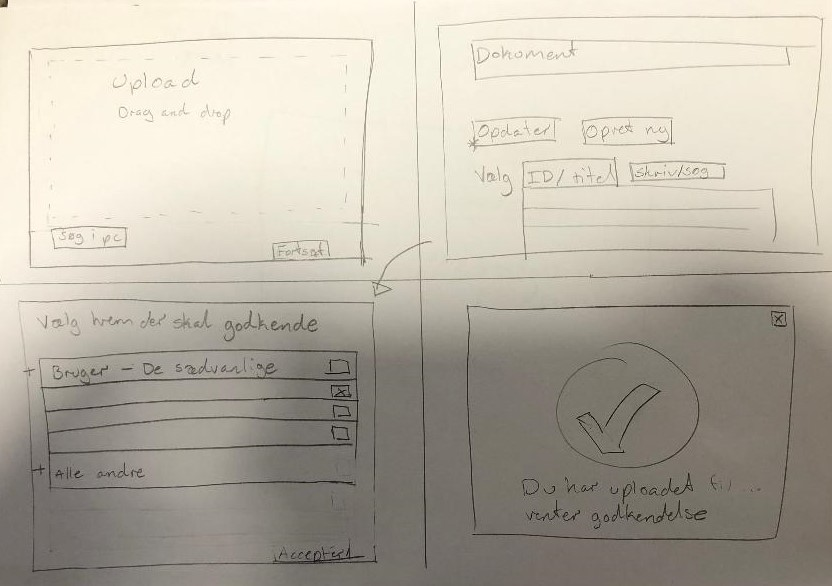
\includegraphics[width=\textwidth]{billeder/Upload-view.jpg}
		\caption{The different interfaces during the upload process}
		\label{fig:1-Upload}
\end{figure}

%Third block of pictures
\begin{figure}[H]
	\centering
	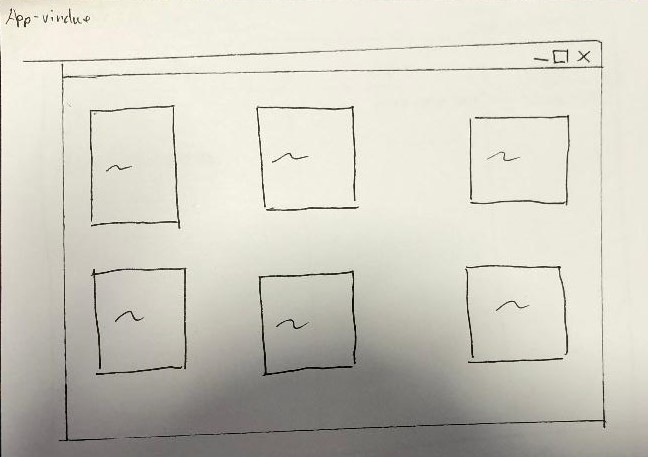
\includegraphics[width=0.5\textwidth]{billeder/app-view.jpg}
	\caption{Interface for first page after login}
	\label{fig:1-app-view}
\end{figure}

\section{Second group of sketches}

\section{prototype for second interview}